
\chapter{The ES-MPT apparatus}

\label{ch:ESMPT}
\comment{here be something}

\section{Superimposed rf and magnetic field}
The problem of particle motion in a \ac{RF} field is by itself
relatively complicated. In the \ac{ES-MPT} we superimpose
the ion-trapping \ac{RF} field with an inhmogeneous magnetic
field for electron guiding, which further increases the complexity
of the particle behavior. In order to assess the feasibility of
running the linear multipole \ac{RF} trap in a weak magnetic field
we investigate briefly the problem of ion motion in a superposition
of \ac{RF} and magnetic field. This problem can be viewed from
many different perspectives, each of which is suitable for
a certain range of physical conditions. Since we do not aim for a
general rigorous treatment, our discussion is based on study
of a specific simple geometry. We will see though, that most
of our observations could be generalized.

Possibly the simplest device featuring inhomogeneous RF electric
field is the cylindrical capacitor --- a hypothetical device
consisting of two infinitely long coaxial cylindrical electrodes.
The electric field between the electrodes follows from the Gauss' law
and is easily expressed in the cylindrical coordinates as
\begin{equation}
\mb E = C_E\frac{\hat {\mb r}}{r},
\label{eq:esmpt:magnetronfield}
\end{equation}
where $\hat{\mb r}$ denotes a unit vector in the direction of the $r$
coordinate. The integration constant $C_E$ is determined by the
electrode dimensions and potentials. The magnetic field $\mb B$ is
homogeneous, constant and parallel to the $z$ axis.

To simplify our discussion, we choose a particular
boundary conditions for electric field and initial conditions
for particle motion. We will vary only the magnetic field
intensity. The following \ac{RF} field
parameters were used:
$C_E = 0.005\;\text{V}$; $\Omega=10\;\text{MHz}$.
Then assuming an \Hminus\ particle starting with zero
initial velocity at a distance of $r_0=50\;\mu\text{m}$ from the
axis, the adiabaticity parameter given by equation
\eqref{eq:trap:adiab} takes the value $\eta\approx 0.15$, which
is safely below the critical threshold $0.3$.
% calc in google
% 2*elementary charge*100 volt/meter*5e-5 meter/(5e-5 meter)^2 / 
% (proton mass*2*pi*(20 megahertz)^2)

An important parameter for describing the interplay of magnetic
and electric fields in determining the particle trajectory is
the ratio of the cyclotron frequency $\omega_c$ to the \ac{RF}
frequency $\Omega$. We denote it as $\Xi$,
\begin{equation}
\Xi = \omega_c/\Omega\,.
\end{equation}

Let us first deal with the conceptually simplest, yet the most
useful case, where $\Xi \ll 1$. In this regime, which corresponds
to the conditions in our experiment, the magnetic
cyclotron oscillations have much larger period than the \ac{RF}
micromotion. In the worst case of \Hminus\ trapping,
the cyclotron frequency at $B=30\;\text{mT}$ is
$\omega_c/2\pi=457\;\text{kHz}$. The coupling between the \ac{RF}
 and cyclotron oscillations is therefore negligible. Since the
magnetic field is small, the assumptions used for derivation
of the effective potential in section \ref{sec:trap} are still
valid. Especially the assumption of micromotion amplitude
depending only on the particle position. By repeating the procedure
for obtaining the effective potential with added Lorentz
force term $q\de\mb r/\de t\times \mb B$ and using the same
ansatz as in the section \ref{sec:trap}, we arrive
at a solution in the form
\begin{equation}
m\frac{\de^2\mb R_0}{\de t^2} =
\frac{q^2}{4m\Omega^2}\nabla\mb E_0^2 +
q\frac{\de \mb R_0}{\de t}\times \mb B\,.
\label{eq:esmpt:secular}
\end{equation}
Here we again obtain an equation completely in terms of the
drift motion, because the contributions of the oscillatory
motion to the Lorentz force vanish by averaging over 1 \ac{RF}
period.

In the special case of the cylindrical magnetron, equation
\eqref{eq:esmpt:secular} can be further solved by observing
that the ponderomotive force is perpendicular to $\mb B$.
The motion is therefore described by the well know drifting
motion in crossed fields, so called $\mb F\times\mb B$ drift.
The \ac{RF} guiding center $\mb R_0$
will perform a cyclotron rotation around a magnetic guiding
center at $\mb R_{\mb B}$, which is in turn orbiting the center
of the magnetron. Here we introduce the terms {\em RF
guiding center} and {\em magnetic guiding center} which
denote the guiding center obtained by averaging over one \ac{RF}
period or over one cyclotron rotation respectively.
The superposition of small scale \ac{RF} micromotion,
intermediate scale cyclotron rotation and large scale drift
motion (also called magnetron motion) is demonstrated in figure
\ref{fig:esmpt:traj}.

\begin{figure}
\centering{
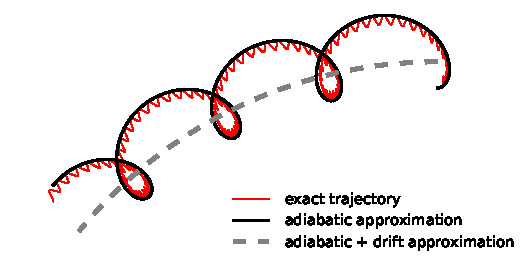
\includegraphics{gfx/trajectory/traj.pdf}
}
\caption{Particle trajectory in a cylindrical \ac{RF} magnetron
for $\Xi\ll 1$.
The exact trajectory is shown as a thin solid red line. The
adiabatic approximation resulting from averaging over one
\ac{RF} period is shown in a thick solid black line. The gyration
center approximation obtained by further averaging the
adiabatic approximation over one cyclotron rotation is shown
as a dashed grey line.}
\label{fig:esmpt:traj}
\end{figure}

Inserting expression for the effective potential
into the general equation of the $\mb F\times \mb B$ 
drift velocity in a non-uniform
effective force field \citep{baumjohan2012} yields an equation
for gyration center motion \comment{unify the terminology - magnetic guiding center, gyration center, cyclotron frequency, Larmor radius, gyroradius, cyclotron radius etc...}
\begin{equation}
\frac{\de \mb R_{\mb B}}{\de t} = 
\frac{q}{4m\Omega^2}
\left(1+\frac{1}{4}r_L^2\Delta\right)
\frac{\nabla\mb E_0^2\times\mb B}{\mb B^2}\,,
\end{equation}
where $r_L$ denotes the Larmor radius.
\comment{define somewhere Larmor radius}
Evaluating this equation
for the magnetron field \eqref{eq:esmpt:magnetronfield} leads
to an analytic expression for the drift velocity
\begin{equation}
\frac{\de \mb R_{\mb B}}{\de t} = 
\frac{q}{2m\Omega^2}
\left(1+\frac{3}{4}\frac{r_L^2}{r^2}\right)
\frac{C_E^2}{r^3\mb B^2}\,.
\end{equation}
The second order term in $r_L/r$ accounting for the electric field
inhomogeneity is usually neglected. In our model problem, it would
change the drift velocity by approximately $1\;\%$.

Finally, we can compare the results of our theoretical analysis with
numerically calculated accurate trajectories.
\comment{Maybe put some more quantitative comparing the different
approaches to calculating the trajectory}.

We have observed that the conclusions of the
adiabatic theory (section \ref{sec:trap}) are still mostly
valid in the case $\Xi \ll 1$.
Just simple modifications are needed to account
for the influence of the magnetic field. Despite the fact, that
only small magnetic field is used in our experimental setup, we
will take at least a qualitative look at the particle behavior
at higher intensities of the magnetic field. Our simulations
show, that a resonant coupling between the \ac{RF} driving
force and cyclotron rotation becomes significant already at
$\Xi\approx0.1$. This coupling is visible as a slight increase
in the particle kinetic energy. Nevertheless, the particle
trajectories still follow the adiabatic approximation within
few percent for $\Xi<0.3$.

As the cyclotron frequency becomes comparable to the excitation
frequency, the adiabatic approximation is not applicable any more.
The presence of {\em beats}, typical for mechanical systems near
resonance is observed, as illustrated by figure \ref{fig:esmpt:beat}.
The figure shows a part of the trajectory for $\Xi = 0.983$.
The particle, starting in the center of the right spiral, is
first spiraling outward due to resonant acceleration. As soon
as the phase difference between the exciting force and the
cyclotron rotation grows to $\pi$, the particle continues
spiraling inward due to resonant deceleration.
\begin{figure}
\centering{
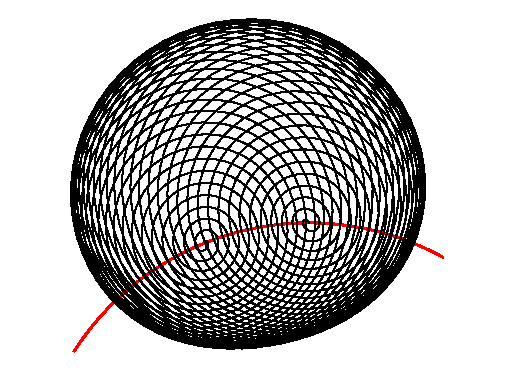
\includegraphics{gfx/trajectory/beats.pdf}
}
\caption{Particle trajectory near resonance, $\Xi=0.98$.
Particle starts with zero initial velocity at maximal amplitude of
\ac{RF} field in the center of the spiral to the right.
One beat period, which consists of resonant acceleration followed
by resonant deceleration, is shown.
The gyration center still follows the magnetron orbit indicated by
the solid red line.
}
\label{fig:esmpt:beat}
\end{figure}

The figure \ref{fig:esmpt:beat} also demonstrates an important
observation, that no matter how much energy the particle
gains by resonant heating, the gyration center always follows
a circular orbit around the magnetron center. The angular
velocity of this
orbiting motion strongly depends on the resonant heating
and even changes direction when crossing the $\Xi=1$ resonance,
but the gyration center never leaves this circle, regardless of
the initial velocity and magnetic field intensity in our simulations.

Finally, the resonance structure
\begin{figure}
\centering{
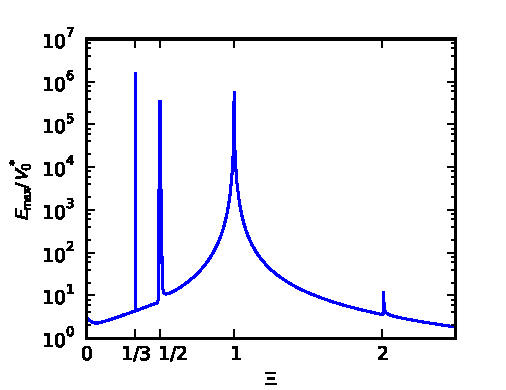
\includegraphics{gfx/resonances/resonances.pdf}
}
\caption{
Resonances
}
\label{fig:esmpt:resonances}
\end{figure}
